%% ma: L10-B15-0092
%% lop: 10
%% chuong: 6
%% bai: 15
%% dang: 10.15.4
%% loai: TN4
%% muc: NB
%% dap_an: "C"
%% nguon: "Ảnh giáo viên gửi 25/11/2026 (lô 2): Bài tập trắc nghiệm – Toán 10 Bài 15 Hàm số (sự biến thiên, đồ thị), Phần I Câu 3"
%% kien_thuc: "Lớp 10 Bài 15 (đồ thị, sự đồng biến, nghịch biến của hàm số)"
%% trang_thai: chinh-thuc
\begin{ex}
Cho hàm số $y=f(x)$ có bảng biến thiên như hình bên dưới. Khẳng định nào sau đây là đúng?
\begin{center}\begin{tikzpicture}\tkzTabInit[lgt=1.2,espcl=3]{$x$/.8,$y$/2}{$-\infty$,$0$,$+\infty$}
\tkzTabVar{-/$-\infty$,+/$1$,-/$-\infty$}
\end{tikzpicture}\end{center}
\choice{Hàm số đồng biến trên khoảng $(-\infty;+\infty)$.}{Hàm số đồng biến trên khoảng $(-\infty;1)$.}{\True Hàm số đồng biến trên khoảng $(-\infty;0)$.}{Hàm số đồng biến trên khoảng $(1;+\infty)$.}
\loigiai{Trên $(-\infty;0)$ mũi tên đi lên nên hàm số đồng biến trên $(-\infty;0)$.}
\end{ex}
